\documentclass[10pt]{article}

\usepackage[margin=0.78in]{geometry}
\usepackage{amsmath}
\usepackage{booktabs}
\usepackage{graphicx}
\usepackage{microtype}
\usepackage[numbers,sort&compress]{natbib}
\usepackage[hidelinks]{hyperref}
\usepackage{xcolor}

% Generated by paper/build_figures.py. Do not edit by hand.
\newcommand{\VarGateRho}{0.37}
\newcommand{\VarGateP}{0.28}
\newcommand{\VarPairRho}{0.26}
\newcommand{\VarColumnR}{0.999}
\newcommand{\CompGateRho}{0.14}
\newcommand{\VarSiteIE}{53.3}
\newcommand{\VarTransferRatio}{1.01}
\newcommand{\CompTransferRatio}{1.00}
\newcommand{\ScaleTransferRatio}{1.02}
\newcommand{\ShortLongRatio}{1.09}
\newcommand{\LongShortRatio}{0.92}
\newcommand{\WrongRatio}{0.59}
\newcommand{\MatchedWrongCos}{0.77}
\newcommand{\EmbedRatio}{0.005}
\newcommand{\AntiIE}{-0.79}
\newcommand{\SelectBestRoute}{46.0}
\newcommand{\TransformRatio}{0.59}
\newcommand{\InstrBestAdd}{20.7}


\title{\textbf{Two Regimes of Linear Steerability:\\
Retrieve/Route Early, Create/Designate Late}}
\author{Sahil Yadav}
\date{July 2026}

\begin{document}
\maketitle

\begin{abstract}
Difference-in-means activation directions are a standard tool for intervening on
language-model behavior. Recent work predicts \emph{which} concepts are linearly
steerable from geometry
\citep{lap2026predicting,geometriccanary2026,whensteerable2026} and can
\emph{generate} steering vectors from natural-language descriptions
\citep{sun2025hypersteer}. What those lines of work do not supply is a
\emph{semantic} account of which \emph{kinds of computation} fall on each side
of the line. We organize four elicited micro-skills in Qwen2.5-7B-Instruct by
computational role---Store, Select, Transform, and Instruction/data
designation---and find a clean two-regime pattern: directions that
\emph{retrieve or route} given information are early and strong (Select
significant at layers 2/8/14, route effect $+\SelectBestRoute$), while
directions that \emph{create or re-designate} meaning are late and weaker
(Transform significant only at 20/26 with ratio $\TransformRatio$ vs store;
Instruction/data significant only at 20/26, add $+\InstrBestAdd$). Deciding
whether text is a command behaves like creating meaning, not retrieving it.
Methodologically we keep the field-standard extraction, pre-register gates and
matched nulls, and treat failed gates as results. A parallel finding---full
patching site-maps fail template replication while residual directions at the
stable site transfer, decompose, and compose---motivates treating
\emph{directions}, not heatmaps, as the reusable object. We position the
two-regime axis as complementary to geometric steerability predictors and to
architectural instruction/data separation \citep{zverev2025aside}: we supply
the missing computational typology, not a new steering mechanism.
\end{abstract}

\section{Introduction}

Activation steering asks whether a residual displacement extracted from
contrastive prompts can be reused to change behavior
\citep{turner2023steering,rimsky2024steering,todd2024function,zou2023representation}.
The extraction recipe we use---difference-in-means at a chosen layer and
token---is deliberately standard
\citep{arditi2024refusal,todd2024function}. The open question in 2026 is not
whether some directions exist, but \emph{which computations admit them}, and
\emph{why}.

Geometric predictors now forecast diff-of-means success from linear
accessibility measures across concept families and models
\citep{lap2026predicting,geometriccanary2026,whensteerable2026}. Separately,
hypernetworks can map a natural-language steering intent to a vector
zero-shot \citep{sun2025hypersteer}. Those results measure and generate
directions; they do not say what \emph{kind of computation} is early-linear
versus late-weak. We address that semantic gap on one controlled primitive
family.

\paragraph{Thesis.}
Linear activation dials are \textbf{early and strong} for
\emph{retrieving/routing} information the model already holds, and
\textbf{late and weak} for \emph{creating or re-designating} meaning.
Instruction-versus-data status---``is this text a command I should obey?''---lands
in the create/designate regime, not the retrieve/route regime.

\paragraph{Also: maps $\neq$ reusable interventions.}
Before the boundary map, we calibrate a methodological warning. Full
layer-by-position patching maps for Variable and Completion fail a
pre-registered template-replication gate, yet residual directions at the
stable site transfer across surfaces, partially decompose past a generic
centroid, and compose within and across skills. Map fragility is therefore not
sufficient evidence of intervention fragility
\citep{hase2023localization,opielka2026invariance}.

\paragraph{Contribution (calibrated).}
We do \emph{not} claim a new steering mechanism, an intent$\to$direction
compiler (taken by HyperSteer), or a general geometric predictor (taken by
LAP). We contribute (i)~a computational-type axis for the steerability
divide, (ii)~a rigorous decompose$\to$compose$\to$boundary arc on one family
with pre-registered nulls, and (iii)~the two-regime finding including
instruction/data. That is a solid complementary paper, not a paradigm founder.

\section{Related work and the 2026 reliability context}

\paragraph{Patching is method-dependent.}
Activation-patching results depend on corruption, intervention direction, and
metric \citep{heimersheim2024patching,zhang2024bestpractices}. Causal scrubbing
and related approaches emphasize testing explicit invariances rather than
reading a single intervention as a complete explanation
\citep{chan2022causal,long2025triangulation}. Our template-disjoint gate follows
that spirit, but evaluates a simpler layer-by-position object. Recent work also
finds substantial variance under paraphrase and resampling
\citep{meloux2025variance}, prompt-specific circuit structure
\citep{franco2026prompt}, and different circuit structures that can implement
interchangeable functions \citep{bayatmakou2026many}. Site fragility is
therefore neither new nor universal.

\paragraph{Activation directions.}
Task and function vectors can compactly mediate in-context functions
\citep{hendel2023task,todd2024function}; activation addition and contrastive
activation addition steer behavior using contrastive residual directions
\citep{turner2023steering,rimsky2024steering,zou2023representation}.
Generalization is uneven across prompts and datasets
\citep{tan2024generalisation,braun2025unreliability}. \citet{nadaf2026steerable}
provide the closest large-scale precedent for cross-template function-vector
transfer; \citet{cheng2026single} instead find that some in-context functions
require coordinated multi-position interventions. Most directly,
\citet{opielka2026invariance} show that causal function vectors need not be
format-invariant and distinguish them from more invariant concept vectors. Our
result is complementary: within a narrow controlled format, the full site-map
is less invariant than the intervention direction extracted at its stable site.
Related dissociations between causal localization and successful manipulation
have also appeared in knowledge editing \citep{hase2023localization}.

\paragraph{Faithfulness warning.}
Successful intervention is not by itself a faithful mechanistic explanation.
Subspace patching can recruit dormant pathways \citep{makelov2024illusion}, and
causal interventions can move representations away from the model's natural
distribution \citep{grant2026divergent}. Our controls reject several simpler
explanations but do not measure representational divergence. We consequently
claim a transferable \emph{intervention direction}, not that the model's unique
natural computation lives in that one-dimensional subspace.

\paragraph{Geometric predictors and intent compilers (what we are \emph{not}).}
\citet{lap2026predicting} and related 2026 work
\citep{geometriccanary2026,whensteerable2026} predict where difference-of-means
steering succeeds from linear-accessibility geometry, with a present-but-nonlinear
versus linearly-steerable regime story. \citet{sun2025hypersteer} generate
steering vectors from natural-language descriptions with zero-shot
generalization. We cite these as the field's geometric and generative frontiers
and do not compete with them: our claim is the missing
\emph{computational typology}---retrieve/route versus create/designate---that
gives semantics to which side of their line a skill occupies.

\paragraph{Instruction/data separation.}
Architectural defenses such as ASIDE rotate data-token embeddings to separate
instructions from data \citep{zverev2025aside}. Probes can detect injection from
activations, and refusal is often one direction \citep{arditi2024refusal}. We
test whether an \emph{obey-versus-quote} residual direction---extracted without
retraining---is strong enough to modulate injection; a weak or null result is
evidence that status designation is not a clean early dial and that architecture
may be necessary.

\section{Experimental setup}

\subsection{Tasks and elicitation}

We use Qwen2.5-Instruct \citep{yang2024qwen25} at 7B (8-bit weights, fp16
residual interventions) and 1.5B (unquantized), with greedy decoding and
chat-templated prompts. Minimal pairs change one computational variable and
have single-token answer alternatives.

\begin{itemize}
    \item \textbf{Binding calibration:} two entity--attribute assignments; the
    counterfactual swaps an answer-relevant attribute.
    \item \textbf{Variable substitution:} ``Let $X=$ dog'' versus ``Let
    $X=$ cat'', followed by a query for $X$. Five variable-name surfaces have
    ten value pairs each.
    \item \textbf{Completion state:} an explicit two-rule table maps a Boolean
    state to one of two actions. Four surface tags have ten instances each.
\end{itemize}

Variable and explicit Completion reach 100\% behavioral accuracy in the retained
sets. An implicit Completion variant without the rule table reaches 0\% and is
excluded. For the later boundary map we add Selection (route among stored
bindings), Transformation ($X{=}X{+}1$), and Instruction/data (obey versus quote
an isolated directive), each behind behavioral gates and matched nulls. A first
Instruction run reported 0\%/0\% elicitation; that verdict was voided after a
leading-space token-id bug in the readout (the model emitted bare tokens). The
same design re-run with bare-token ids cleared Stage~1 (100\%/75\%) before any
causal claim. Failed gates and 0\% readouts trigger a harness-bug hunt before a
scientific null.

\subsection{Patching and map replication}

For clean input $x$ and counterfactual $x'$, let $h_{\ell,p}$ denote the
post-layer residual at layer $\ell$, position $p$. We patch
$h_{\ell,p}(x)\leftarrow h_{\ell,p}(x')$ and measure
\[
  \mathrm{IE}_{\ell,p}
  = d\!\left(x;h_{\ell,p}\leftarrow h_{\ell,p}(x')\right)-d(x),
\]
where $d=\operatorname{logit}(a_{\mathrm{cf}})
-\operatorname{logit}(a_{\mathrm{clean}})$ at the final position. Logit
difference is continuous and approximately linear in the residual stream, as
recommended for patching studies \citep{heimersheim2024patching}.

The pre-registered P1 gate computes maps on template-disjoint halves and
requires Spearman $\rho>0.5$ and superiority to a pair-partition null at
$p<0.01$. A random-position null separately tests the expected site.

\subsection{Direction transfer}

At a frozen layer and slot, donor templates define
\[
  \Delta = \frac{1}{n}\sum_i
  \left(h_{\ell,p}(x'_i)-h_{\ell,p}(x_i)\right).
\]
We add $\alpha\Delta$ to clean held-out targets. A target cell passes when
(i) mean $\Delta$IE is positive, (ii) it beats 100 same-norm random directions
at $p<0.01$, and (iii) cross-template $\Delta$IE divided by a direction learned
within that target is at least 0.5. Primary tests use $\alpha=1$ and layer 2,
frozen from the 7B maps.

\section{Results}

\subsection{The instrument recovers a known causal site}

On 30 entity--attribute Binding pairs at 7B, patching the queried entity's
attribute position moves answer log-odds in the predicted direction against a
matched random-position null ($p=0.001$). The effect replicates on two disjoint
15-pair halves (both $p=0.001$), and the top site is the known changed
attribute. This calibration blocks the explanation that downstream failures are
caused by a nonfunctional harness.

\subsection{Sharp site-maps fail template replication}

Both novel skills fail P1. Variable has a large expected-site effect
($\mathrm{IE}=\VarSiteIE$, $p=0.001$) and a sharp top site at layer 2,
position 27, yet its template-half map correlation is only
$\rho=\VarGateRho$ ($p=\VarGateP$). Completion has
$\rho=\CompGateRho$; its top effect is at position 62, one token after the
pre-registered bit at position 61.

The Variable failure is specifically about the full map. Across all ten
template pairs, mean full-grid correlation is \VarPairRho, while the
expected-position column alone correlates at \VarColumnR{} (Figure
\ref{fig:coordinate}). A stable causal column sits inside non-replicating
off-site geometry. ``Map failure'' here always means failure under this frozen
full-grid scoring rule; it does not imply that every semantically aligned site
description is unstable.

\begin{figure}[t]
    \centering
    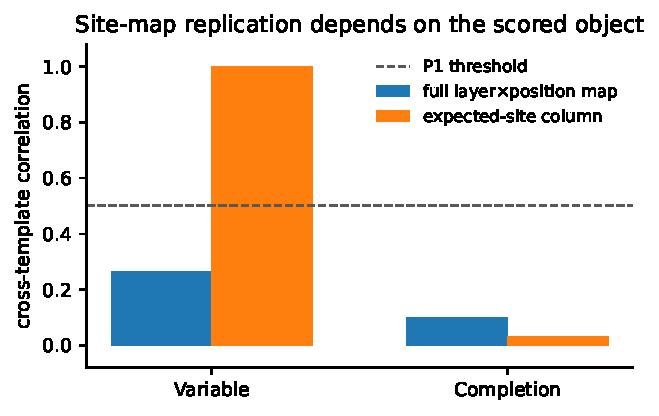
\includegraphics[width=0.72\linewidth]{figures/coordinate_system.pdf}
    \caption{\textbf{The scored object changes the replication verdict.}
    Pairwise correlations across Variable and Completion surfaces. Variable's
    full maps are fragile while its value-position column is nearly identical
    across surfaces. The dashed line is the pre-registered P1 threshold.}
    \label{fig:coordinate}
\end{figure}

\subsection{Directions transfer where maps do not}

For Variable at 7B, a direction from surfaces $X,Y$ transfers to held-out
$Z,W,K$ with ratios $1.04,1.14,0.83$ (mean \VarTransferRatio), each beating its
same-norm random-direction null. Leave-one-surface-out transfer has mean ratio
$1.07$.

The result generalizes in three pre-registered ways (Figure
\ref{fig:transfer}). First, Completion direction transfer from surfaces $A,B$ to
$C,D$ at the map's top position yields mean ratio \CompTransferRatio{} and flips
the greedy answer on every target. The bit position itself has zero direction
norm, consistent with the map peak occurring one token later. Second, Variable
at 1.5B passes all three held-out surfaces at layer 2 with mean ratio
\ScaleTransferRatio. Third, an inert prefix moves the Variable slot from
position 27 to 40; short-to-long and long-to-short directions both pass all
targets, with mean ratios \ShortLongRatio{} and \LongShortRatio.

\begin{figure}[t]
    \centering
    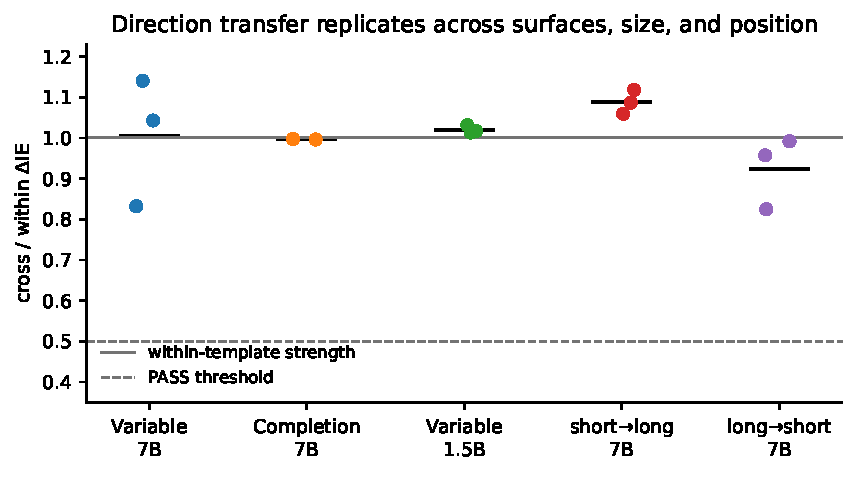
\includegraphics[width=0.88\linewidth]{figures/transfer_ratios.pdf}
    \caption{\textbf{Held-out transfer relative to a within-surface direction.}
    Points are target surfaces; black ticks are means. Every primary cell clears
    the pre-registered 0.5 ratio and random-direction significance gates.
    Completion was tested at 7B; the Variable protocol was replicated
    separately at both model sizes.}
    \label{fig:transfer}
\end{figure}

\subsection{Controls identify a coarse slot update}

At 7B, the Variable result is stable for $\alpha=1,2$ and for layers 1--4 at
$\alpha=1$; $\alpha=0.5$ fails the all-target gate. Greedy flips begin only at
$\alpha\geq3$, which we treat as strong steering rather than mechanism evidence.

An input-embedding difference added at the layer-0 output passes zero of three
targets and has only \EmbedRatio{} of the layer-2 cross effect. Thus the useful
direction is computed beyond the token embedding. Adding the negative matched
direction produces mean $\Delta$IE=\AntiIE, establishing sign sensitivity.

The decisive caveat is a re-forwarded wrong-value control. We replace each
donor's counterfactual with an unrelated value, recompute the layer-2 direction,
and test held-out transfer. It still passes all targets at mean ratio
\WrongRatio{} and has cosine \MatchedWrongCos{} with the matched direction
(Figure \ref{fig:controls}), triggering the pre-registered
\texttt{GENERIC\_BOOST} verdict. The matched vector therefore contains a large
generic component. The exact supported interpretation is a coarse
``update this value slot'' intervention, not a direction carrying a specific
lexical binding.

\begin{figure}[t]
    \centering
    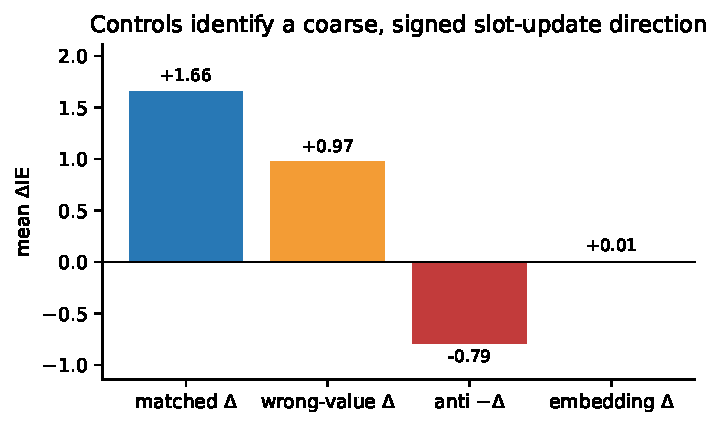
\includegraphics[width=0.72\linewidth]{figures/controls.pdf}
    \caption{\textbf{Controls set the claim strength.} Mean held-out $\Delta$IE
    for the matched, unrelated-value, negative, and embedding directions. The
    wrong-value effect is real but weaker; the negative direction hurts; the
    embedding difference is negligible.}
    \label{fig:controls}
\end{figure}

\subsection{A value-specific residual survives removal of the generic direction}

The \texttt{GENERIC\_BOOST} verdict concerns the \emph{aggregate} direction,
which averages over all ten value transitions. We instead build \emph{per-value}
directions $\Delta_v=\frac{1}{5}\sum_{i:\,a_{\mathrm{cf}}=v}
\big(h_{\ell,p}(x'_i)-h_{\ell,p}(x_i)\big)$ at layer~2 and the value slot, and
measure, on held-out prompts, both transfer (does $\Delta_v$ raise $v$'s logit)
and \emph{selectivity} $s(v)=\Delta\!\operatorname{logit}(v)-\operatorname{mean}_{w\neq v}\Delta\!\operatorname{logit}(w)$.

The per-value directions are approximately orthogonal: mean pairwise cosine is
$0.01$ (near the $\sqrt{9/3584}\approx0.05$ chance level for a nine-dimensional
subspace), and each $\Delta_v$ aligns with the aggregate at cosine $\approx0.32$,
the value expected for ten orthogonal equal-norm vectors and their mean
($\sqrt{10}/10$). The generic-looking aggregate is thus quantitatively consistent
with being their centroid rather than a separate dominant mechanism. The
value-specific residual (each $\Delta_v$ minus its projection onto the span of
the other nine directions) transfers and is value-selective for all ten values
(mean transfer $+8.8$, mean selectivity $+8.7$, each $p<0.01$ against same-norm
random directions), while the norm-matched generic component is weakly selective
($+0.6$).

We then run a pre-registered \emph{centroid-removal} control: subtract the single
empirical generic direction $\hat g\propto\sum_v\Delta_v$ from each $\Delta_v$
and re-measure. The value-selective effect survives for all ten values (mean
selectivity $+5.9$, $p<0.01$), so a value-specific component exists beyond the
generic direction. The centroid is not inert, however: norm-matched selectivity
retention is median $0.85$ (below our pre-registered $0.90$), heterogeneous
across values (largest loss for the values whose direction most overlaps the
centroid), and the centroid added alone is non-selective ($+0.03$). We therefore
report \texttt{CENTROID\_MATTERS}: value-specific and generic components coexist
and are not fully separable. (The residual retains $\approx99\%$ of the norm,
which is partly high-dimensional geometry; selectivity, not norm, is the
evidence.)

\subsection{Directions compose within and across skills}

Independently validated directions can be added simultaneously and retain their
effects. \emph{Within skill}: in a two-variable prompt (``Let $X=\ldots$
Let $Y=\ldots$''), installing $X$'s value direction at $X$'s slot and $Y$'s at
$Y$'s slot at once retrieves both values selectively (each $p<0.01$), with
retention $\approx1.0$ relative to installing one alone and cross-talk near zero
(installing $Y$ does not raise $X$'s target). \emph{Across skills}: in one prompt
that contains both a Variable binding and an explicit Completion rule with a bit,
adding the Variable value direction and the heterogeneous Completion bit
direction at their respective layer-2 sites steers both readouts independently
--- value selectivity $+9.4$ and Completion action log-odds $+39.0$, each
$p<0.01$, retention $\approx1.0$, cross-talk near zero (the value direction does
not flip the action, and the bit direction does not install a value). These
micro-skill directions therefore act as approximately independent, composable
interventions at this site. Given that composition of steering/function vectors
is often unreliable \citep{todd2024function,tan2024generalisation}, the clean
within- and cross-skill composition is notable, though it remains
sufficiency-and-steerability evidence rather than a claim about the model's
unique circuit.

\subsection{Two regimes of linear steerability}

With transferable directions in hand, we ask which \emph{computations} admit
early, strong dials. Four skills, one family, pre-registered layer sweeps
$\{2,8,14,20,26\}$ and same-norm nulls:

\begin{center}
\begin{tabular}{@{}lll@{}}
\toprule
Regime & Skills & Profile \\
\midrule
Given information (hold \& route) & Store, Select & early, strong \\
Derived / created meaning & Transform, Instruction/data & late, weak \\
\bottomrule
\end{tabular}
\end{center}

Select clears significance at layers 2/8/14 (best route $+\SelectBestRoute$) and
is null late. Transform's computed-value direction is significant only at 20/26
(ratio $\TransformRatio$ vs the store control). Instruction/data---$\Delta$ from
obey versus quote frames of the same directive---is significant only at 20/26
(add-to-data $+\InstrBestAdd$; ablate signed correctly), with early layers null.
Figure~\ref{fig:tworegimes} shows the normalized accessibility curves: retrieve/route
clusters early; create/designate clusters late. The non-obvious claim is that
\emph{designating text as a command} patterns with \emph{creating} a value, not
with \emph{routing} among stored bindings.

\begin{figure}[t]
    \centering
    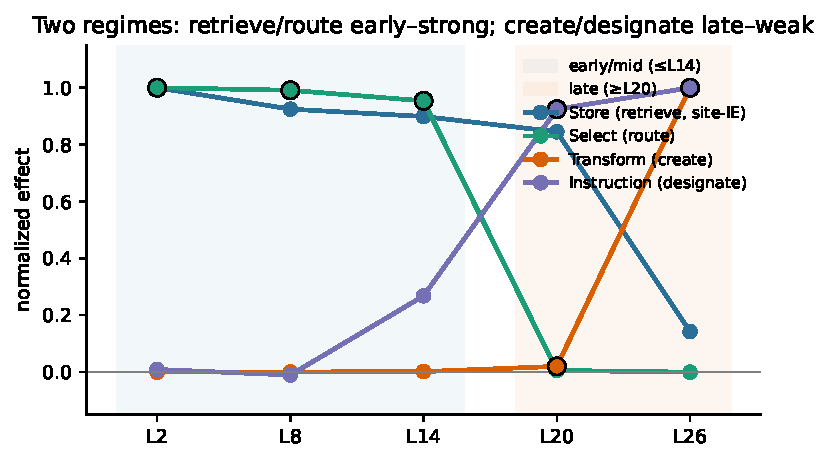
\includegraphics[width=0.88\linewidth]{figures/two_regimes.pdf}
    \caption{\textbf{Two regimes of linear steerability.} Normalized per-layer
    effects for Store (Variable site-IE at the expected position), Select
    (routing), Transform (computed-value selectivity), and Instruction/data
    (add $\Delta_{\mathrm{instr}}$ to data-framed prompts). Filled markers:
    layers that pass the pre-registered null gate (Store marker: primary
    direction-transfer site). Retrieve/route peaks early; create/designate only
    late.}
    \label{fig:tworegimes}
\end{figure}

\paragraph{Injection control (Stage~3).}
At the significant Instruction layers, $\pm\Delta_{\mathrm{instr}}$
\emph{partially} modulates a single-token prompt-injection readout (embedded
directive inside a quotation). Adding $\Delta$ raises injection logit-difference
significantly at layers 20 and 26 (greedy injection rate $0\%\to50\%$ / $25\%$),
but the full pre-registered dial fails: ablation at 20 misses $p<0.01$, and
ablation at 26 costs 38pp of clean utility. We report
\texttt{INJECTION\_PARTIAL}: obey-status steering moves injection but is
insufficient alone as a defense, consistent with architectural separation
\citep{zverev2025aside}. We do not fish after the failed full dial.

\section{Discussion}

\paragraph{Semantics for a geometric divide.}
LAP-style predictors answer \emph{whether} a concept is linearly accessible;
we answer \emph{what kind of computation} tends to be. The two-regime axis is
therefore complementary, not competing
\citep{lap2026predicting,sun2025hypersteer}. Intent$\to$direction generation is
HyperSteer's. We pre-registered a type$\to$profile prediction on two held-out
skills (boolean NOT as route$\to$early; numeric comparison as
create$\to$late). Both were elicitable, and the gate
\texttt{TYPOLOGY\_FALSIFIED}: NOT never formed an early dial under the tested
$\Delta$, and comparison peaked late but also reached significance at layer~14.
The four-skill observation therefore remains an organized pattern, not yet a
confirmed predictive typology---an honest negative we retain.

\paragraph{A coordinate-system result.}
The conventional map and the direction answer different questions. P1 asks
whether the complete scalar effect geometry over sites survives a template
change. Direction transfer asks whether a displacement extracted at a selected
site can be reused elsewhere. In our tasks, the first fails and the second
passes at roughly within-surface strength. Therefore, rejecting the map is not
enough to reject reusable activation-space interventions.

\paragraph{What ``position-free'' means here.}
The Variable direction transfers between positions 27 and 40 after an inert
prefix. This rules out dependence on one absolute token index. It does not show
invariance to arbitrary instruction format, language, tokenizer, or model
family. This distinction is important given evidence that causally effective
function vectors can remain format-specific \citep{opielka2026invariance}.

\paragraph{What remains mechanistically unresolved.}
Our controls show a layer-computed, signed effect and reject equal-norm random
directions. They do not prove that activation addition follows the model's
natural computational path. In particular, we do not measure whether
$h+\Delta$ remains on the natural latent distribution
\citep{grant2026divergent}, nor do we rule out dormant-pathway recruitment
\citep{makelov2024illusion}. ``Transferable intervention direction'' is
therefore the strongest justified term. Transform and Instruction being
\emph{weak} is part of the result, not an omission.

\paragraph{From coarse slot update to composable primitives.}
Per-value directions recover a value-selective residual that survives removal of
the empirical generic direction, and independently validated directions compose
within and across skills with near-zero cross-talk. The early/strong regime is
where that composition story is cleanest; the late/weak regime marks where
linear dials thin out.

\section{Limitations}

The tasks are synthetic prompt-level micro-skills in one model family
(Qwen2.5), mostly at 7B with 8-bit weights. The two-regime claim rests on four
skills; a pre-registered typology prediction on held-out skills
(\texttt{TYPOLOGY\_FALSIFIED}) did not upgrade that pattern to a confirmed
predictive theory. Store's curve in
Figure~\ref{fig:tworegimes} uses site-IE for comparability of shape; Select,
Transform, and Instruction use direction-add effects---metrics are normalized
within skill, not equated across skills. Injection Stage~3 is
\texttt{INJECTION\_PARTIAL} on a single-token synthetic embedding of a
directive, not a full adaptive attack suite. We do not claim cross-model vector
transfer, natural-manifold faithfulness, or that directions are the model's
unique circuit. Extraction is standard difference-in-means; novelty is the axis
and the rigor. With 100 random directions, primary control $p$-values are
resolution-limited at $1/101\approx0.0099$.

\section{Conclusion}

Linear dials on this primitive family split by computational role:
\textbf{retrieve/route is early and strong; create/designate is late and weak.}
Instruction/data designation joins Transform on the late side. The same project
shows that fragile patching site-maps need not imply fragile interventions:
directions at the stable site transfer, partially decompose, and compose. We
position this as the semantic complement to geometric steerability predictors
and intent-conditioned generators---a trustworthy typology paper in a crowded
field, not a new steering paradigm.

\bibliographystyle{plainnat}
\bibliography{references}

\end{document}
